\chapter{Diseño}\label{cap:disenio}

En este capitulo se documentara como se desarrollo el diseño de la arquitectura del proyecto, para ello se expondrá el modo en que trabaja \jd y además se mostrara la estructura de clases que se eligió para el sistema para que pueda cumplir con los requisitos expuestos en el Capitulo \ref{capitulo:especificacion}.





\section{Visión general}

Para diseñar \jj como ya se menciono se tomo como base a el patrón de desarrollo DAO que se explico en la sección \fullref{jdbgm:dao}, siguiendo la idea de este patrón \jj debe manejar todas las consultas echas a el motor por lo que la aplicación solo se deberá comunicar con \jj para acceder a el motor de base de datos, se puede observar esquemáticamente esta idea en la figura \figpage{fig:jdbgm:overview} en la que podemos observar que la idea es que la aplicación utilice el formato que estamos proponiendo para trabajar con las sentencias SQL, estas serán interpretadas por \jj y convertidas a una cadena de texto la cual es entendible por \jd y este se comunicara directamente con el DBMS y pondrá a disposición de \jj el resultado que dependiendo de la consulta puede ser un objeto del tipo \verb=ResultSet= o un tipo \verb=integer=. 

\begin{figure}
  \centering
    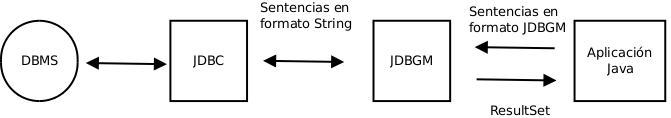
\includegraphics[width=0.85\textwidth]{figuras/jdbgm-overview.png}
  \caption{JDBGM dentro de una aplicación}
  \label{fig:jdbgm:overview}
\end{figure}

Así que \jj debe ser capaz de hacer dos tareas independientes pero relacionadas, en primer lugar debe proveer el almacenamiento de las sentencias de modo que puedan ser traducidas luego a el dialecto que corresponda y en segundo lugar proveer los métodos necesarios para comunicarse con el motor mediante \jd, podemos observar esquemáticamente la situación en la figura \figpage{fig:jdbgm:closerlook} que nos muestra la idea de independencia existente entre los dos módulos principales que se están exponiendo, el manejador de sentencias es totalmente independiente de la capa intermedia pues de lo que esta encargado es de proveer los métodos necesarios para "armar las sentencias" y traducirlas cuando sea requerido a el dialecto correspondiente, esta traducción lo que hace es convertir la sentencia almacenada a una cadena de texto la cual es entendible por \jd por lo que se podría obviar la capa intermedia que hace transparente su uso y usarlo directamente. En cambio la capa intermedia dependerá de el manejador de sentencias para poder proveer la independencia de dialectos que se quiere lograr y además este solo recibirá las sentencias compatibles con el formato propuesto por \jj por lo que a continuación se procederá a explicar la estructura propuesta para este manejador para que después se pueda explicar correctamente el funcionamiento de la capa intermedia.

\begin{figure}
  \centering
    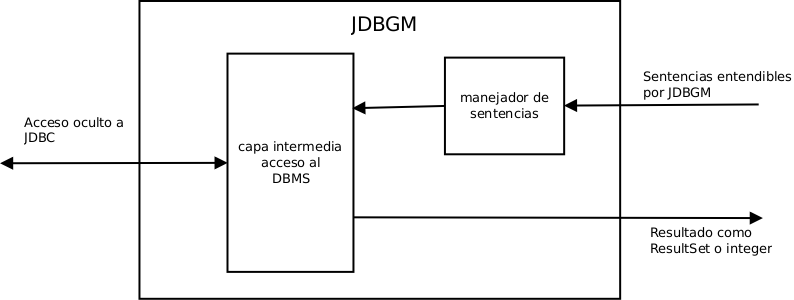
\includegraphics[width=0.85\textwidth]{figuras/jdbgm-closerlook.png}
  \caption{Vista abstracta del funcionamiento de JDBGM}
  \label{fig:jdbgm:closerlook}
\end{figure}

\subsection{Manejador de sentencias}

Java ya nos provee JDBC para acceder a las bases de datos, pero al hacer uso de el es necesario especificar con que motor se esta trabajando, para ejemplificar ello veamos el típico código que debemos escribir para conectarnos a una base de datos.

\begin{lstlisting}[title=Porción de codigo java para la conexión a una base de datos]
class conectDB(){
...

Class.forName("com.mysql.jdbc.Driver");
	Connection conexion = DriverManager.getConnection(
		"jdbc:mysql://localhost/AsistenciaAlumnos", "tester",
		"tester");
	Statement st = (Statement) conexion.createStatement();

...
}
\end{lstlisting}

En esta porción de código lo que se hace inicialmente es instanciar el driver, es decir crear el objeto driver, luego el método estático \verb=getConnection= de 	\verb=DriverManager= nos devuelve un objeto que representa la conexión al motor con el que se esta trabajando. Este objeto del tipo \verb=Connection= nos provee métodos para generar objetos \verb=Statement= que nos permite hacer consultas a la base de datos mediante las funciones que dispone. Una descripción mucho mas extensa de JDBC puede ser encontrada en la documentación disponible en la web de Oracle\citep{java:jdbc}.
Para nuestro proyecto necesitamos ocultar y simplificar el API de JDBC




\section{JDBC y su envoltorio}
y otro






\section{Abstracción de SQL}
